%! TEX root = ../thesis.tex

\chapter{Neural networks}
\label{chap:neural-networks}

The idea of a \textbf{N}eural \textbf{N}etwork (NN) is to attempt to capture the human thinking process in machine code. For this purpose, a network architecture
connects some input (e.g. a picture) to an output (e.g. digits 0-9). Much like in a human brain, the architecture consists of multiple smaller chunks, neurons 
and layers, which connect in some way to form an emergent intelligent system. 

As described, neural network do not yet hold the abilities to achieve their designated tasks, and can hardly be called intelligent. They need to be trained. 
This is done by presenting an example input (called training data) to the network. The network output is compared to the desired output for the given input via 
some loss function. During training, the network attempts to minimize this loss function. How it is minimized is often a design choice, and in general will 
depend on the network architecture, which in turn is influenced by the type of data and kind of task the NN should accomplish.

In the following several network architectures which are relevant for this work are detailed. The most simple option of a \textbf{D}ense NN (DNN) is given in 
\autoref{sec:DNN} in order to introduce several key concepts. \textbf{C}onvolutional NNs (CNNs) used for example in image recognition are explained in 
\autoref{sec:CNN}. Lastly \textbf{R}ecurrent NNs (RNNs) that find an application in time series analysis are shown in \autoref{sec:RNN}

\section{Dense neural network}
\label{sec:DNN}

Dense neural networks are subdivided into layers, which themselve consist of individual neurons. Each neuron conglomerates information from a previous layer 
according to some weights $w_{jk}$ and a bias $b_j$ and propagates it through some nonlinear activation function $\sigma^{(i)}$. That is, the propagation of 
an input to the output layer through intermediate, hidden layers $\mathcal{L}^{(i)}$ can be described with the below matrix form:

\begin{equation}
\label{eq:dnn-propagation}
\mathcal{L}_j^{\,(i)} = \sum\limits_{k = 0}^{n^{(i-1)}} \sigma^{(i)}\left( w_{jk} \mathcal{L}_j^{\,(i-1)} + b_j\right).
\end{equation}

In \autoref{eq:dnn-propagation} $\mathcal{L}_j^{\,(i)}$ is the value of neuron $j$ in layer $i$, and $n^{(i)}$ is a reference to the number of neurons in 
layer $i$. The activation function achieves two important goals. First, it limits the numerical value neurons can have. This ensures numerical stability
during training, and is typically achieved by choosing a sigmoidal activation function. Secondly, the nonlinearity of the activation function ensures that 
the propagation function of the entire network cannot mathematically be reduced to a single layer, as this disallows the network to learn nonlinearly 
separable patterns \cite{russell2010artificial}. 

Important to note is the fact that the usage of one densely connected layer does not restrict the network architecture to consist solely of such layers. 
In fact, the network architectures discussed here and in the following section can all be used interchangably. This is a common practice in model building
\cite{szegedy2015going, krizhevsky2017imagenet}.


\section{Convolutional neural network}
\label{sec:CNN}

Convolutional neural networks introduce convolutional layers, which aggregate information from nearby input values. Nearby in this case referring for example 
to proximate pixels in a 2D image, or neighbouring voxels in a 3D scan. Even succesive inputs in a 1-dimensional time series can be convoluted. In general, 
the working principle of a convolutional layer can be extended to an arbitrary input shape and size, but will be representatively explained here for a 
two-dimensional, image-like input.

The convolution in a single layer is done by one or several filters, matrices, that are scalar-multiplied to subchunks of the input data. For example a mock 
filter like

\begin{figure}[H]
	\centering
	\begin{subfigure}[h]{0.45\linewidth}
		\begin{equation*}
			\resizebox{\hsize}{!}{\ensuremath{
				\mathcal{F} = 
				\begin{pmatrix}
				-1 & -1 & -1 & -1 & -1 & -1 \\
				-1 & +1 & -1 & -1 & +1 & -1 \\
				-1 & -1 & -1 & -1 & -1 & -1 \\
				-1 & +1 & -1 & -1 & +1 & -1 \\
				-1 & +1 & +1 & +1 & +1 & -1 \\
				-1 & -1 & -1 & -1 & -1 & -1
				\end{pmatrix}
			}}
		\end{equation*}
	\end{subfigure}
	\hfill
	% \vspace{-40cm}
	\begin{subfigure}[h]{0.45\linewidth}
	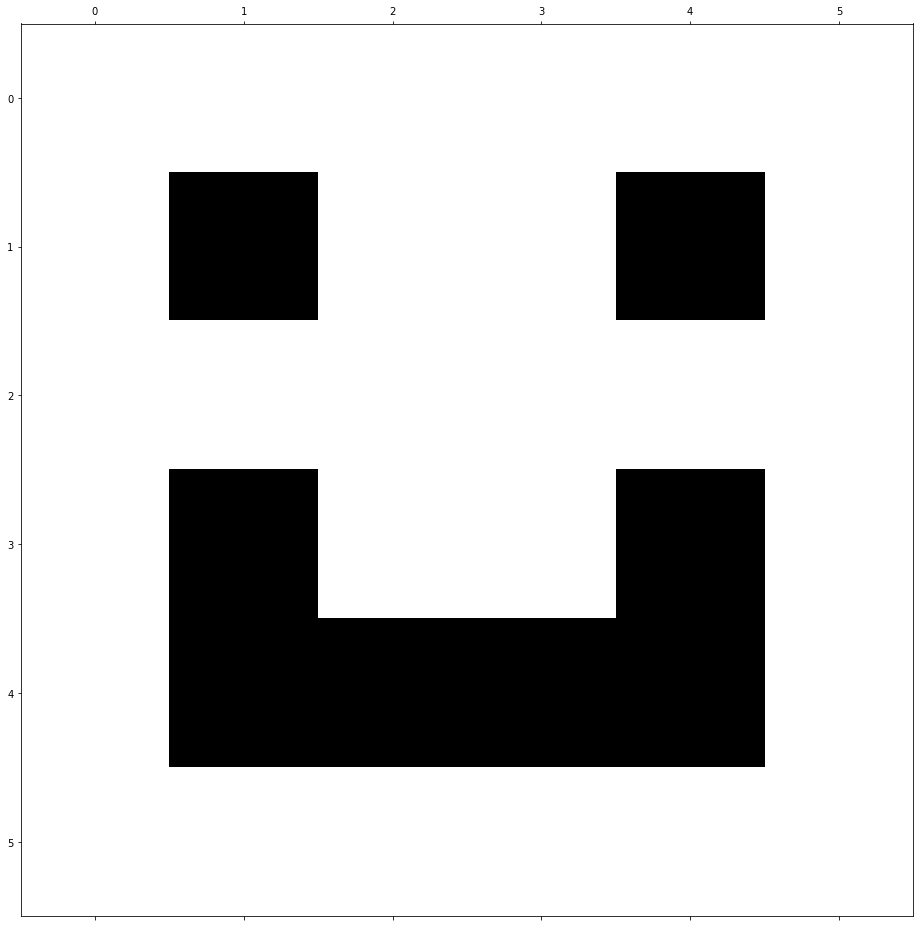
\includegraphics[height=4.2cm]{imgs/convolution.png}
	\end{subfigure}
\end{figure}


could be swept across an entire image area. During the iteration, areas of the image that resemble the filter will result in a large (relative to the input data)
positive scalar value.

In this fashion, an image can be efficiently scanned for specific patterns (lines, edges, etc.) with just few parameters. Namely, these are the numerical
values in the filter matrices, which can be optimized during training. The resulting output of a single layer containing different filters can interatively 
be propagated into subsequent convolutional layers (searching for curves, corners, etc.) until full-scale image detection of complex structures becomes possible.

\section{Recurrent neural network}
\label{sec:RNN}

Recurrent neural networks not only propagate an input value forward through their architecture, but also introduce cyclic connections between distinct layers. For
example, in the simplest conceptional case there exists a feedback loop that connects the output of a single network layer to its' input(c.f. 
\autoref{fig:simple-RNN}). Other feedback configurations are of course possible, and generally preferred, as they can address the problem of vanishing/exploding 
gradients \cite{hochreiter1991untersuchungen}. 

Moreover, due to the cyclic connections in the network architecture, RNNs are espically qualified for time-series analysis. i.e. where temporally sucessive inputs
are highly correlated. A popular example is the \textbf{L}ong \textbf{S}hort-\textbf{T}erm \textbf{M}emory (LSTM) architecture, which is visualized in 
\autoref{fig:LSTM}.

\begin{figure}
	\centering
	\begin{subfigure}[h]{0.45\linewidth}
	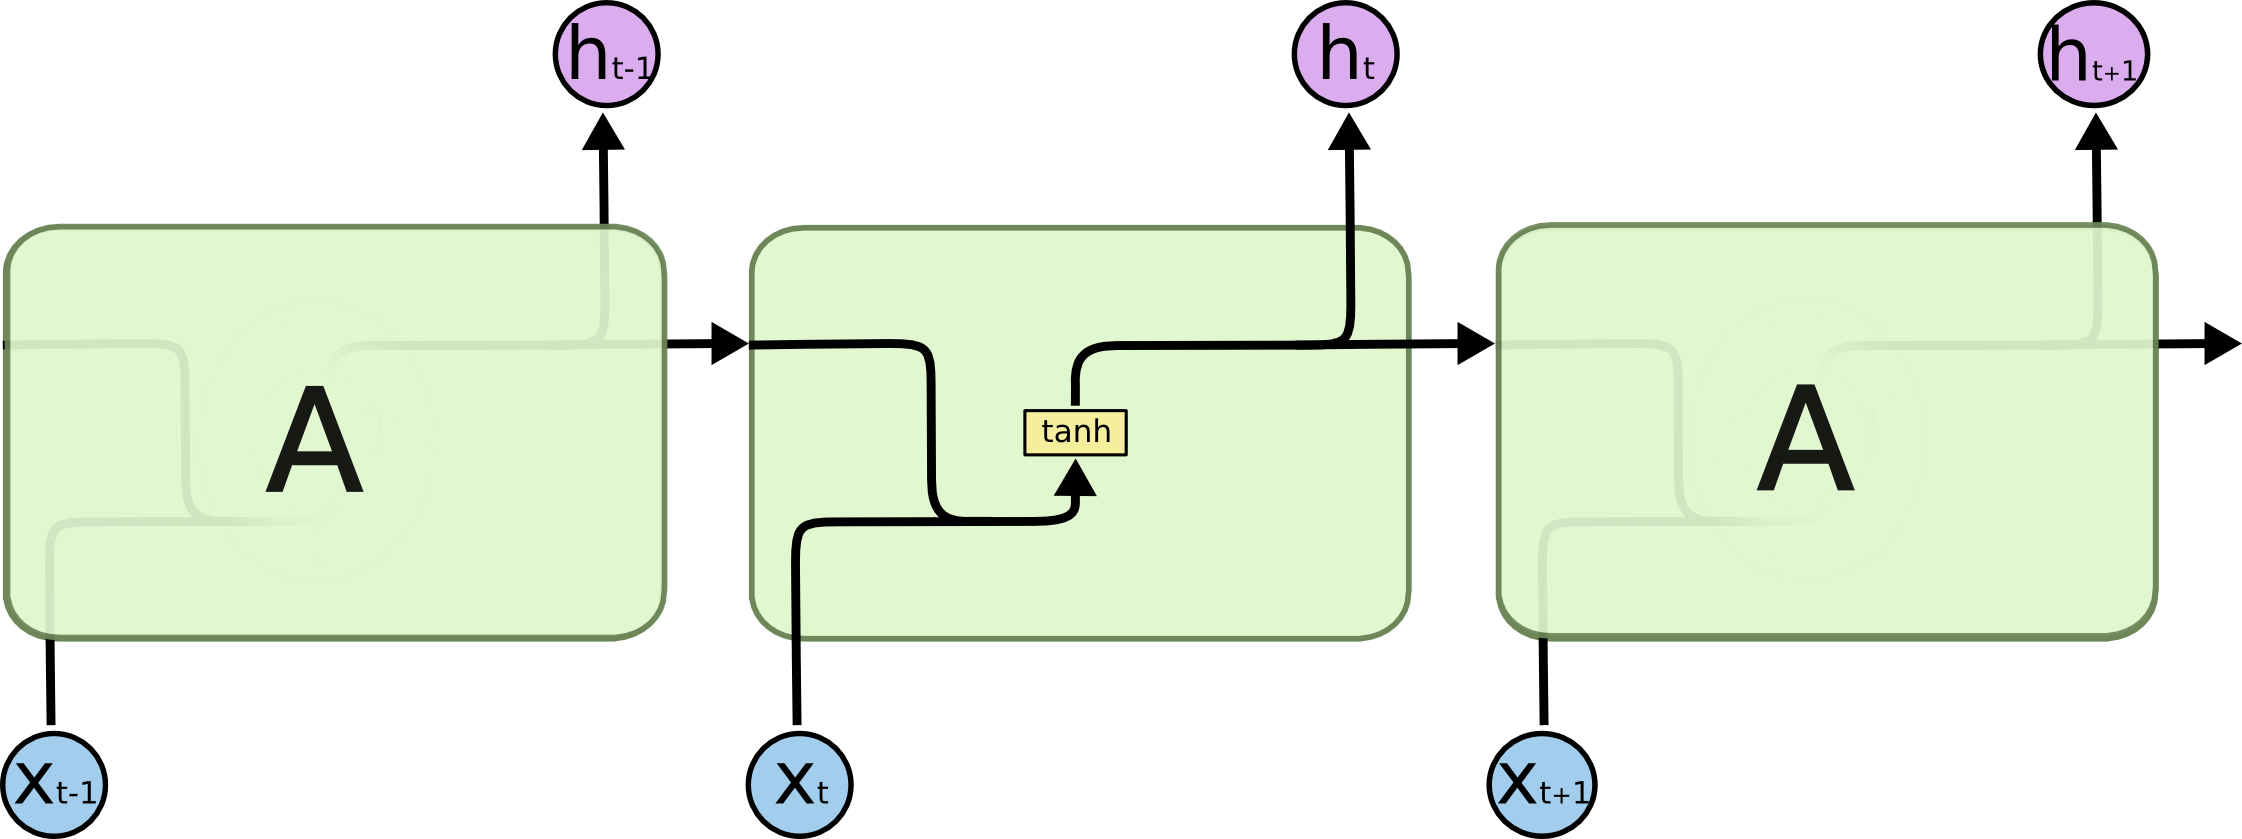
\includegraphics[height=4.2cm]{imgs/simple_RNN.png}
	\caption{\textbf{simple RNN}\label{fig:simple-RNN}}
	\end{subfigure}
	% \hfill
	% \vspace{-40cm}
	\begin{subfigure}[h]{0.45\linewidth}
	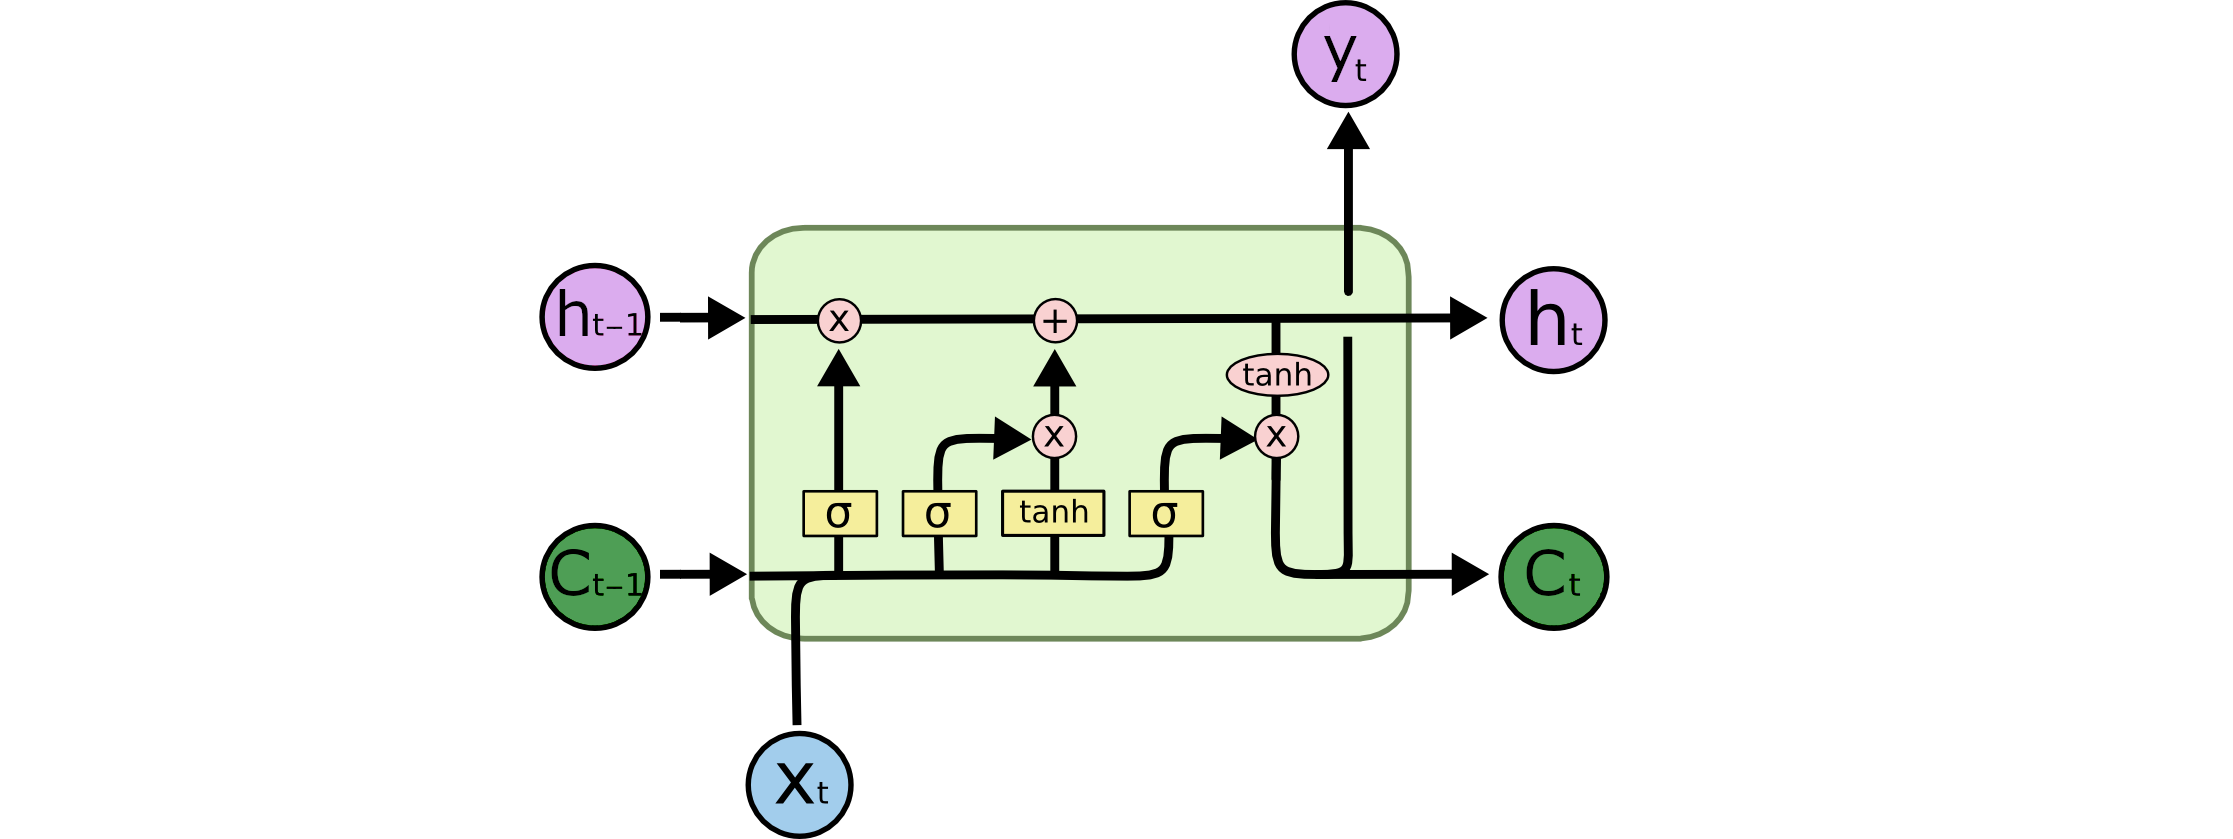
\includegraphics[height=4.2cm]{imgs/LSTM.png}
	\caption{\textbf{LSTM}\label{fig:LSTM}}
	\end{subfigure}
	\caption*{\textbf{a)} An example RNN architecture, with one layer A, where the network output $h_t$ of at step $t$ is used as an additional input for step $t+1$. 
	Image altered from \cite{NN-images}. \textbf{b)} The architecture of a single LSTM layer relies on multiple gates, that update the network configuration, or 
	memory of the layer. From \cite{NN-images} with changes. \label{fig:NN-architectures}.}
\end{figure}

The output of a single LSTM layer at timestep $t\neq0$ is calculated from two variables, the hidden state $h_t$, as well as the cell state $C_t$. The former exists in 
some form in every RNN, while the cell state $C_t$ corresponds to a long-term memory that is unique to the LSTM architecture \cite{gers2000learning}. Unlike the name 
implies, the hidden state corresponds to the output of the network, and is thus in no way hidden. Due to vanishing/exploding gradients, the hidden state does not 
preserve information for more than few iterations. For this reason, it is often referred to as the short-term memory of the network. Data propagates through an LSTM 
layer according to the below steps (c.f. as well \autoref{fig:LSTM}):

\begin{itemize}
	\item A sigmoid layer outputs a number between 0 and 1 depending on the input $x_t$. The cell state from the previous iteration, $C_{t-1}$, is weighted by this 
	number. In this fashion, the network can choose to discard or keep information from previous iterations. The first sigmoid layer is thus aptly named the 
	forget gate.
	\item Next, the new cell state is calculated by extracting important information from the input. This is achieved via a feature extraction layer, which is 
	weighted by another instance of a sigmoidal layer. The thus recovered new long term memory is added to the weighted cell state $C_{t-1}$ and represents the new 
	cell state $C_t$. This is the input gate of the LSTM.
	\item Lastly, the hidden state $h_t$ is computed at the output gate of the LSTM. A feature extraction layer processes $C_t$ and provides an output, that is 
	weighted by one last sigmoid layer dependant on the input $x_t$.
\end{itemize}

\section{Other architectures}
\label{sec:NN-other}

With the current rise of deep learning applications in every facet of data processing, a plethora of other architectures have been established to achieve specific
tasks. Some of these are purely generative (e.g. \textbf{G}enerative \textbf{A}dversarial \textbf{N}etworks (GANs) \cite{creswell2018generative}) or not out of the 
box suitable for classification due to other reasons. Of particular interest, specifically for this work, are architectures that have been shown to outperform others
in time-series analysis. Apart from the LSTM discussed in \autoref{sec:RNN} the \textbf{G}ated \textbf{R}ecurrent \textbf{U}nit (GRU) \cite{dey2017gate} is a popular 
implementation of a recurrent neural network. Last but not least, transformers \cite{vaswani2017attention} have consistently been among the most promising architectures 
for time-series analysis. However, because they require a lot of computational resources they are not compatible with the use-case that this work is pertaining to.